\documentclass[tikz,border=2pt]{standalone}
\usepackage{tikz,amsmath,amssymb}
\usetikzlibrary{arrows.meta}
\begin{document}
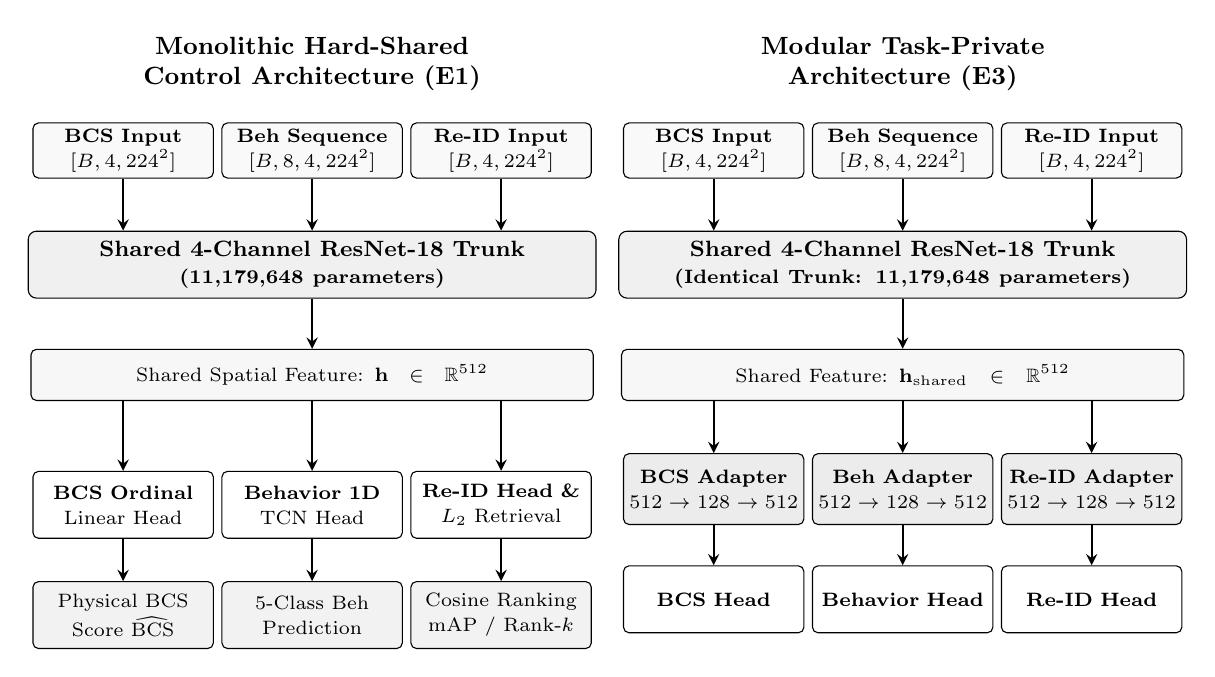
\begin{tikzpicture}[
  title/.style={font=\bfseries\small, align=center},
  inbox/.style={draw, rectangle, rounded corners=2pt, align=center, font=\scriptsize, text width=2.15cm, minimum height=0.7cm, fill=gray!5, inner sep=2pt},
  trunk/.style={draw, rectangle, rounded corners=3pt, align=center, font=\footnotesize\bfseries, text width=7.0cm, minimum height=0.85cm, fill=gray!12, inner sep=3pt},
  feat/.style={draw, rectangle, rounded corners=2pt, align=center, font=\scriptsize, text width=7.0cm, minimum height=0.65cm, fill=gray!6, inner sep=2pt},
  adapter/.style={draw, rectangle, rounded corners=2pt, align=center, font=\scriptsize, text width=2.15cm, minimum height=0.9cm, fill=gray!15, inner sep=2pt},
  head/.style={draw, rectangle, rounded corners=2pt, align=center, font=\scriptsize, text width=2.15cm, minimum height=0.85cm, inner sep=2pt},
  outbox/.style={draw, rectangle, rounded corners=2pt, align=center, font=\scriptsize, text width=2.15cm, minimum height=0.85cm, fill=gray!10, inner sep=2pt},
  arrow/.style={->, >=stealth, thick}
]

% ==================== LEFT: Hard-Shared MTL ====================
\node[title] at (3.75, 1.1) {Monolithic Hard-Shared\\Control Architecture (E1)};

\node[inbox] (e1_in1) at (1.35, 0.0) {\textbf{BCS Input}\\[1pt]$[B, 4, 224^2]$};
\node[inbox] (e1_in2) at (3.75, 0.0) {\textbf{Beh Sequence}\\[1pt]$[B, 8, 4, 224^2]$};
\node[inbox] (e1_in3) at (6.15, 0.0) {\textbf{Re-ID Input}\\[1pt]$[B, 4, 224^2]$};

\node[trunk] (e1_trunk) at (3.75, -1.45) {Shared 4-Channel ResNet-18 Trunk\\{\scriptsize (11,179,648 parameters)}};

\draw[arrow] (e1_in1.south) -- (e1_in1 |- e1_trunk.north);
\draw[arrow] (e1_in2.south) -- (e1_trunk.north);
\draw[arrow] (e1_in3.south) -- (e1_in3 |- e1_trunk.north);

\node[feat] (e1_feat) at (3.75, -2.85) {Shared Spatial Feature: $\mathbf{h} \in \mathbb{R}^{512}$};
\draw[arrow] (e1_trunk) -- (e1_feat);

\node[head] (e1_h1) at (1.35, -4.5) {\textbf{BCS Ordinal}\\[1pt]Linear Head};
\node[head] (e1_h2) at (3.75, -4.5) {\textbf{Behavior 1D}\\[1pt]TCN Head};
\node[head] (e1_h3) at (6.15, -4.5) {\textbf{Re-ID Head \&}\\[1pt]$L_2$ Retrieval};

\draw[arrow] (e1_feat.south -| e1_h1.north) -- (e1_h1.north);
\draw[arrow] (e1_feat.south) -- (e1_h2.north);
\draw[arrow] (e1_feat.south -| e1_h3.north) -- (e1_h3.north);

\node[outbox] (e1_o1) at (1.35, -5.9) {Physical BCS\\[1pt]Score $\widehat{\mathrm{BCS}}$};
\node[outbox] (e1_o2) at (3.75, -5.9) {5-Class Beh\\[1pt]Prediction};
\node[outbox] (e1_o3) at (6.15, -5.9) {Cosine Ranking\\[1pt]mAP / Rank-$k$};

\draw[arrow] (e1_h1) -- (e1_o1);
\draw[arrow] (e1_h2) -- (e1_o2);
\draw[arrow] (e1_h3) -- (e1_o3);

% ==================== RIGHT: Modular Task-Private MTL ====================
\node[title] at (11.25, 1.1) {Modular Task-Private\\Architecture (E3)};

\node[inbox] (e3_in1) at (8.85, 0.0) {\textbf{BCS Input}\\[1pt]$[B, 4, 224^2]$};
\node[inbox] (e3_in2) at (11.25, 0.0) {\textbf{Beh Sequence}\\[1pt]$[B, 8, 4, 224^2]$};
\node[inbox] (e3_in3) at (13.65, 0.0) {\textbf{Re-ID Input}\\[1pt]$[B, 4, 224^2]$};

\node[trunk] (e3_trunk) at (11.25, -1.45) {Shared 4-Channel ResNet-18 Trunk\\{\scriptsize (Identical Trunk: 11,179,648 parameters)}};

\draw[arrow] (e3_in1.south) -- (e3_in1 |- e3_trunk.north);
\draw[arrow] (e3_in2.south) -- (e3_trunk.north);
\draw[arrow] (e3_in3.south) -- (e3_in3 |- e3_trunk.north);

\node[feat] (e3_feat) at (11.25, -2.85) {Shared Feature: $\mathbf{h}_{\mathrm{shared}} \in \mathbb{R}^{512}$};
\draw[arrow] (e3_trunk) -- (e3_feat);

\node[adapter] (ad1) at (8.85, -4.3) {\textbf{BCS Adapter}\\[1pt]$512 \to 128 \to 512$};
\node[adapter] (ad2) at (11.25, -4.3) {\textbf{Beh Adapter}\\[1pt]$512 \to 128 \to 512$};
\node[adapter] (ad3) at (13.65, -4.3) {\textbf{Re-ID Adapter}\\[1pt]$512 \to 128 \to 512$};

\draw[arrow] (e3_feat.south -| ad1.north) -- (ad1.north);
\draw[arrow] (e3_feat.south) -- (ad2.north);
\draw[arrow] (e3_feat.south -| ad3.north) -- (ad3.north);

\node[head] (e3_h1) at (8.85, -5.7) {\textbf{BCS Head}};
\node[head] (e3_h2) at (11.25, -5.7) {\textbf{Behavior Head}};
\node[head] (e3_h3) at (13.65, -5.7) {\textbf{Re-ID Head}};

\draw[arrow] (ad1) -- (e3_h1);
\draw[arrow] (ad2) -- (e3_h2);
\draw[arrow] (ad3) -- (e3_h3);

\end{tikzpicture}
\end{document}